\section{Filter and Activation Visualizations — Minimal CNN}
\label{sec:Filter and Activation Visualizations — Minimal CNN}

%\smash{% Your over-sized minipage... from % https://tex.stackexchange.com/questions/397746/preventing-minipage-from-creating-a-blank-page
% scale some images by 0.8 fixed the blank page on page 14
    \begin{figure}[H]
        \centering
        \begin{minipage}[t]{0.55\textwidth}
            \vspace{-22.5em}
            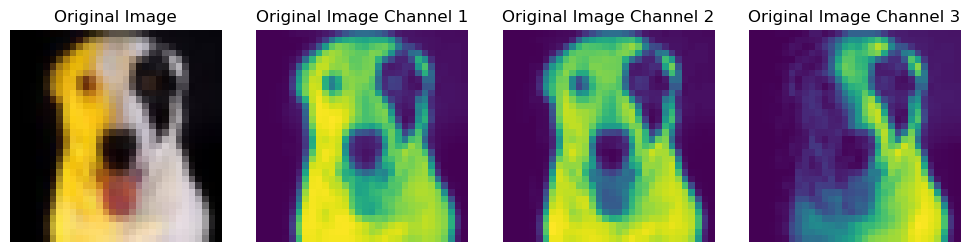
\includegraphics[width=\linewidth]{Plots/Appendix_B/cifar_image.png}
            \centering\subcaption*{(a) CIFAR-10 image and its RGB channels with R~=~1, G~=~2 and B~=~3.}
            \vspace{1em}

            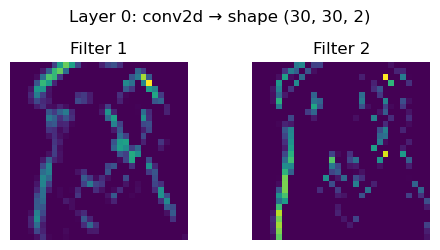
\includegraphics[width=0.8\linewidth]{Plots/Appendix_B/cifar_image_after_filter.png}
            \centering\subcaption*{(b) Feature maps after first Conv2D layer with 2 Filters (CIFAR-10).}
            \vspace{1em}

            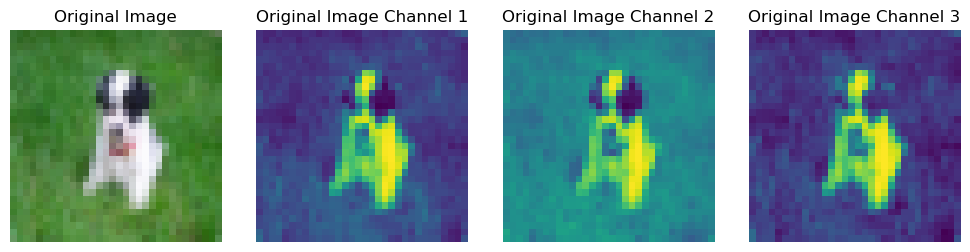
\includegraphics[width=\linewidth]{Plots/Appendix_B/imageNet_image.png}
            \centering\subcaption*{(c) ImageNet image and its RGB channels with R~=~1, G~=~2 and B~=~3.}
            \vspace{1em}

            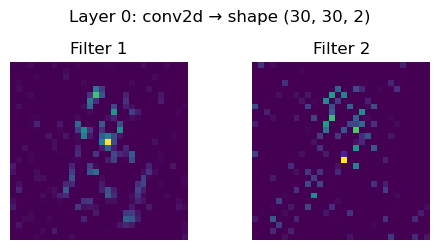
\includegraphics[width=0.8\linewidth]{Plots/Appendix_B/imageNet_image_after_filter.png}
            \centering\subcaption*{(d) Feature maps after first Conv2D layer with 2 Filters (ImageNet).}
        \end{minipage}
        \hfill
        \begin{minipage}[t]{0.35\textwidth}
            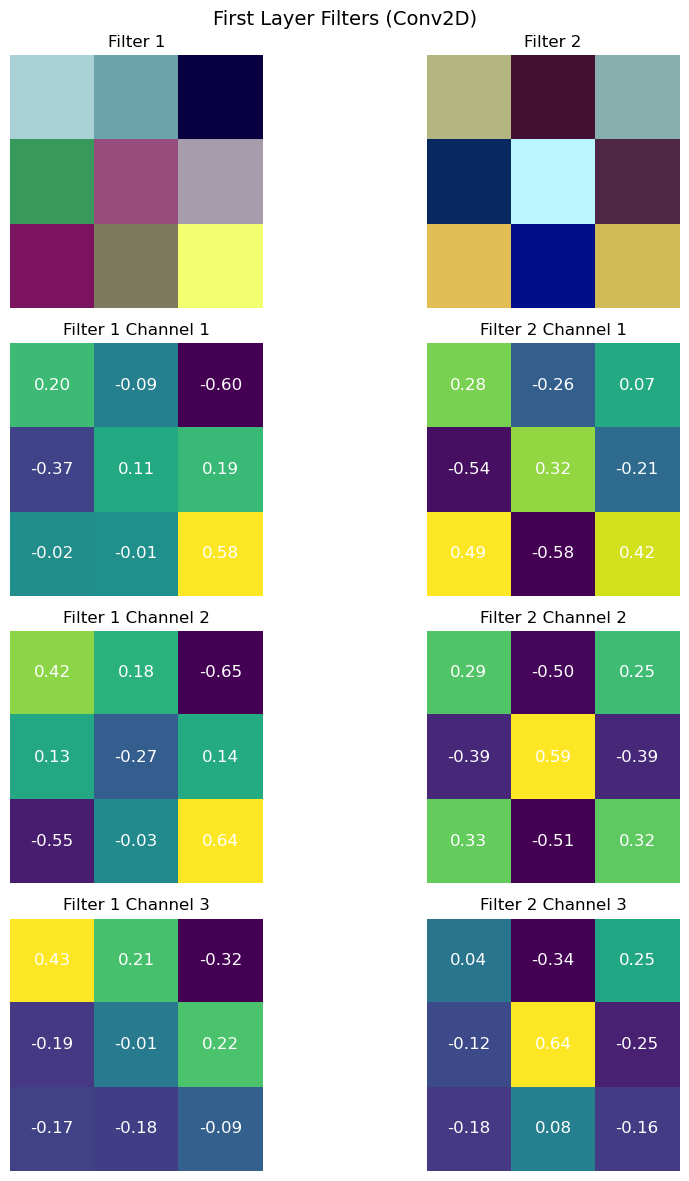
\includegraphics[width=\linewidth]{Plots/Appendix_B/Kernels_minimal_model.png}
            \centering\subcaption*{(e) First Conv2D layer filters of the Minimal Model mentioned in \autoref{subsec: Minimal CNN for Visualization} (3 channels, 3 × 3) where Channel 1, 2 and 3 correspond to R, G and B in that order.}
        \end{minipage}
        \caption{Overview of the input images, intermediate feature maps after the first convolutional layer and learned kernels of the minimal CNN model.}
    \end{figure}
%}